% ============================================================
% Appendix C — TikZ Operator Tables for NDH & Fun-Sphere Physics
% Fun-Sphere Fantasy Engine — Preprint Figures
% Location: fun-sphere-fantasy-engine/preprints/figures/
% Author: Borealis S. Hedling
% Date: October 2026
% ============================================================

\documentclass[tikz,border=10pt]{standalone}
\usepackage{tikz}
\usetikzlibrary{matrix, positioning, arrows.meta}

\begin{document}

% ============================================================
% C.1 NDH Altitude Operators Table
% ============================================================
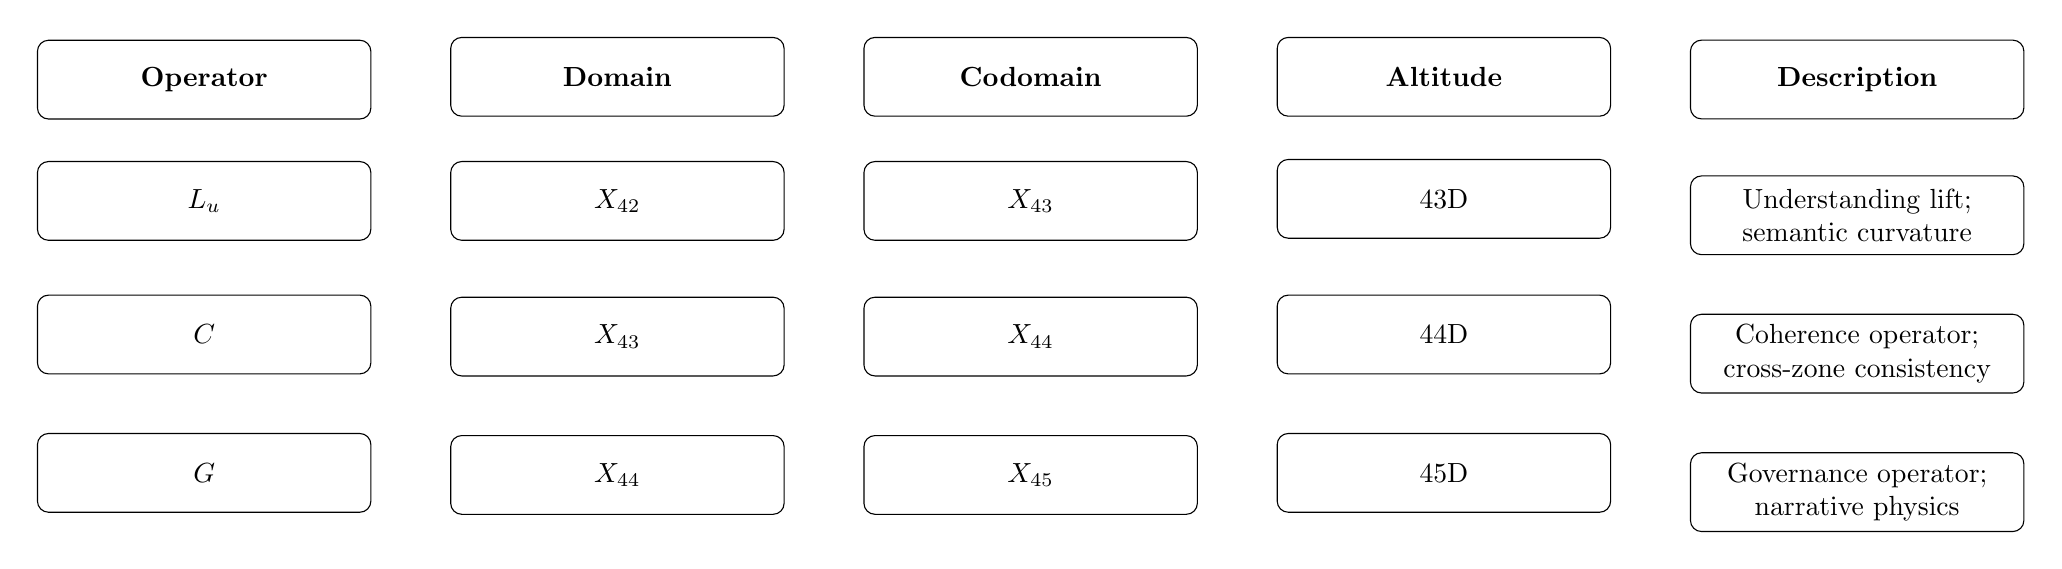
\begin{tikzpicture}
\matrix (m) [matrix of nodes,
    nodes={draw, rectangle, rounded corners, align=center, text width=4cm, minimum height=1cm},
    column sep=1cm, row sep=0.5cm
]{
\textbf{Operator} & \textbf{Domain} & \textbf{Codomain} & \textbf{Altitude} & \textbf{Description} \\
$L_u$ & $X_{42}$ & $X_{43}$ & 43D & Understanding lift; semantic curvature \\
$C$ & $X_{43}$ & $X_{44}$ & 44D & Coherence operator; cross-zone consistency \\
$G$ & $X_{44}$ & $X_{45}$ & 45D & Governance operator; narrative physics \\
};
\end{tikzpicture}

\vspace{1.5cm}

% ============================================================
% C.2 NDH Interpretation Algebra Operators (42D)
% ============================================================
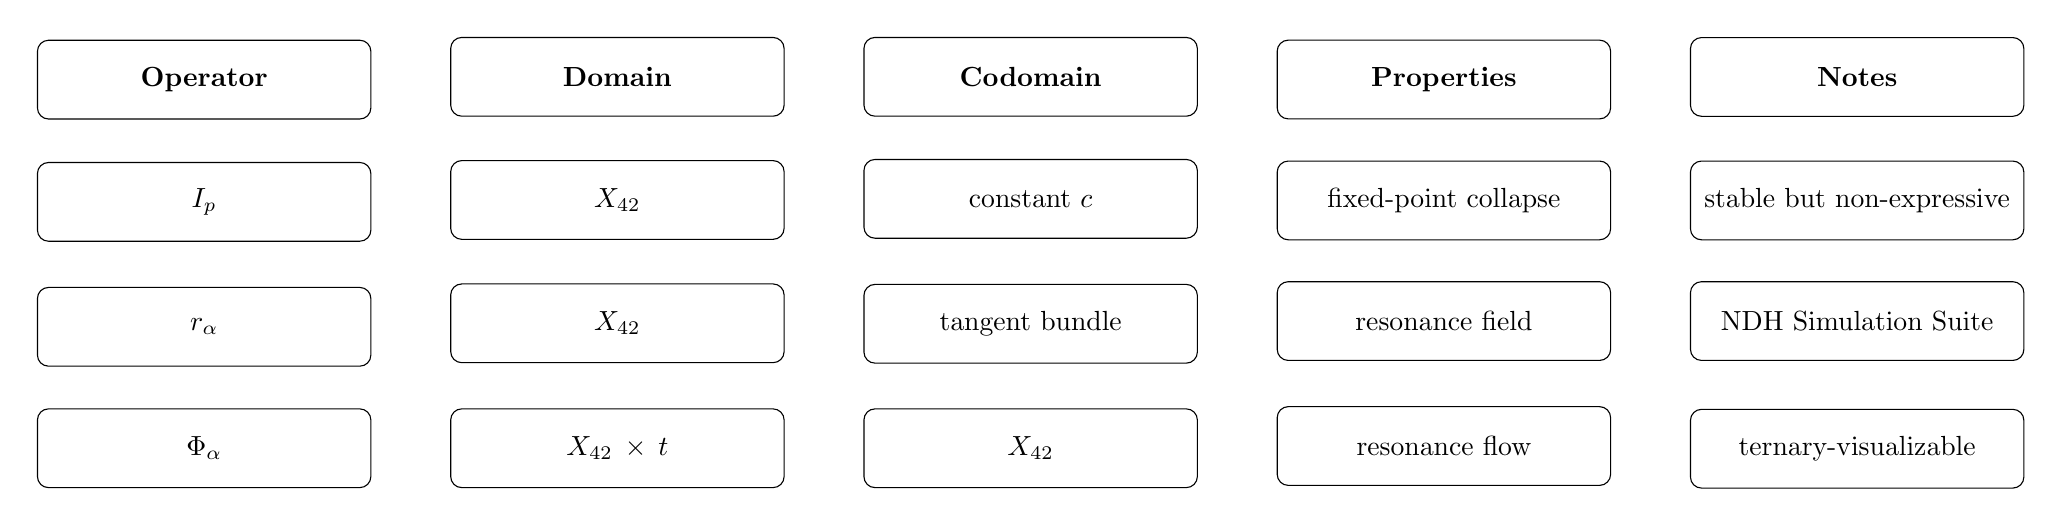
\begin{tikzpicture}
\matrix (m2) [matrix of nodes,
    nodes={draw, rectangle, rounded corners, align=center, text width=4cm, minimum height=1cm},
    column sep=1cm, row sep=0.5cm
]{
\textbf{Operator} & \textbf{Domain} & \textbf{Codomain} & \textbf{Properties} & \textbf{Notes} \\
$I_p$ & $X_{42}$ & constant $c$ & fixed-point collapse & stable but non-expressive \\
$r_\alpha$ & $X_{42}$ & tangent bundle & resonance field & NDH Simulation Suite \\
$\Phi_\alpha$ & $X_{42} \times t$ & $X_{42}$ & resonance flow & ternary-visualizable \\
};
\end{tikzpicture}

\vspace{1.5cm}

% ============================================================
% C.3 Ternary Projection Operators
% ============================================================
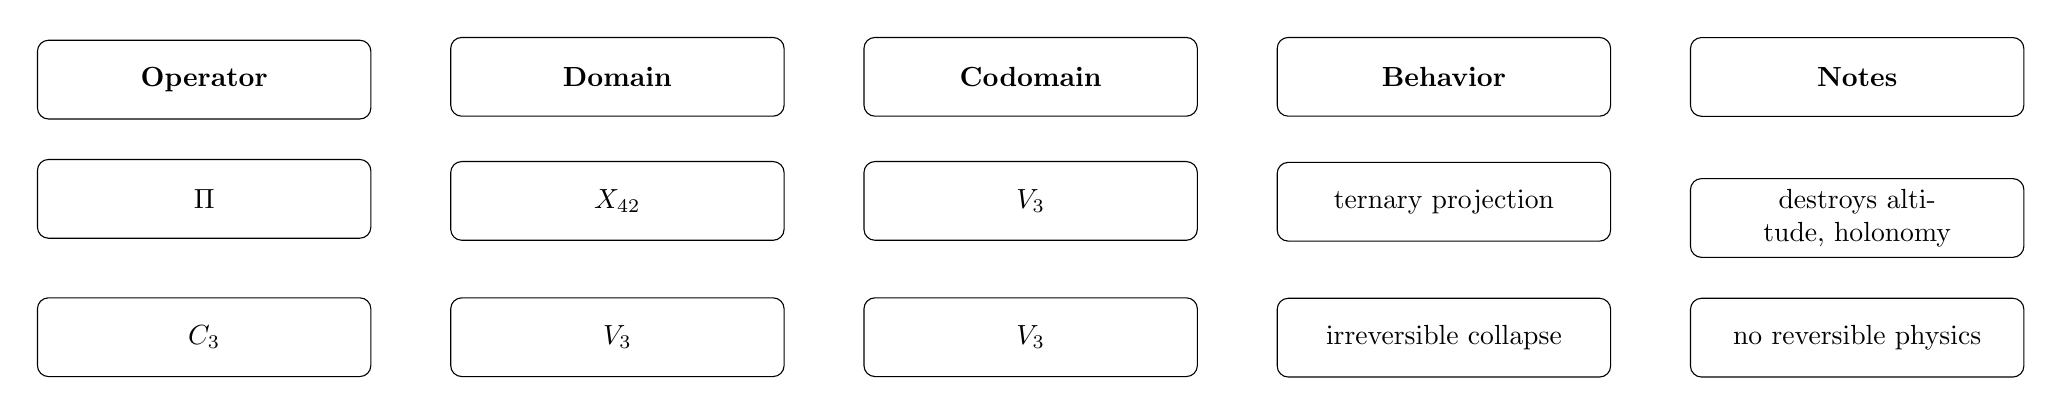
\begin{tikzpicture}
\matrix (m3) [matrix of nodes,
    nodes={draw, rectangle, rounded corners, align=center, text width=4cm, minimum height=1cm},
    column sep=1cm, row sep=0.5cm
]{
\textbf{Operator} & \textbf{Domain} & \textbf{Codomain} & \textbf{Behavior} & \textbf{Notes} \\
$\Pi$ & $X_{42}$ & $V_3$ & ternary projection & destroys altitude, holonomy \\
$C_3$ & $V_3$ & $V_3$ & irreversible collapse & no reversible physics \\
};
\end{tikzpicture}

\vspace{1cm}

\begin{tikzpicture}
\node[draw, rectangle, rounded corners, align=center, text width=10cm, padding=6pt] {
$C_3(u \otimes_3 v \otimes_3 w) = C_3(u)$ \\[4pt]
$\Pi \circ R_\theta = \Pi$
};
\end{tikzpicture}

\vspace{1.5cm}

% ============================================================
% C.4 Holonomy Operators
% ============================================================
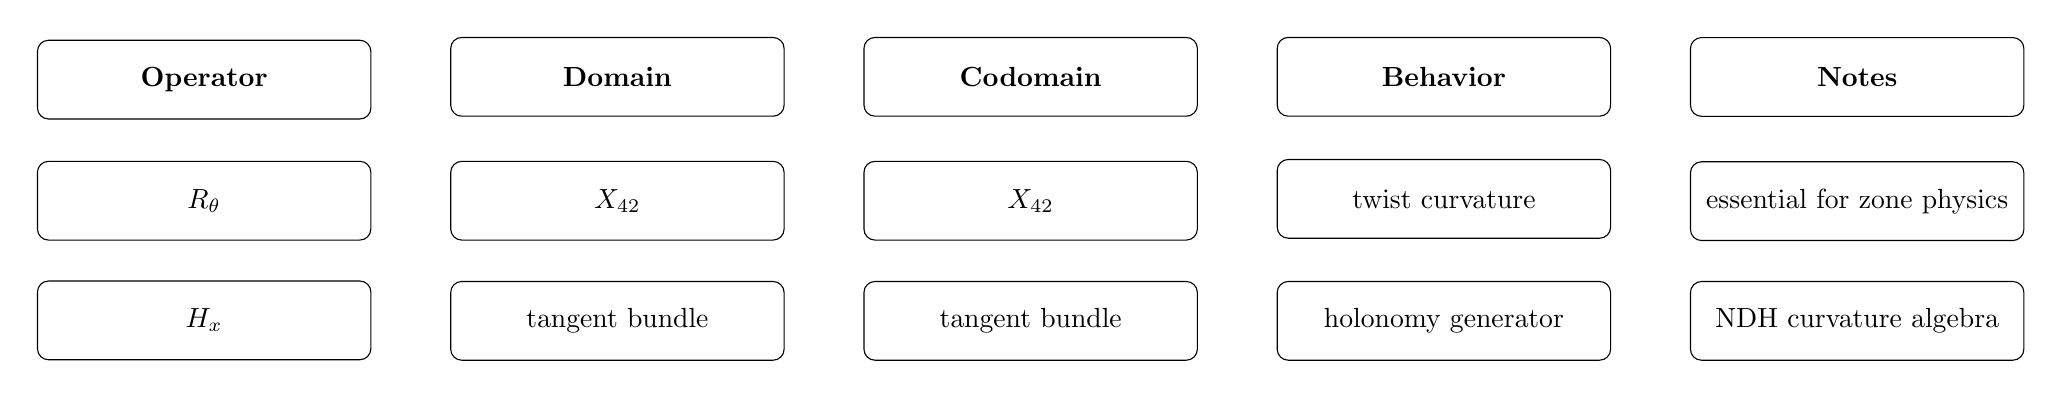
\begin{tikzpicture}
\matrix (m4) [matrix of nodes,
    nodes={draw, rectangle, rounded corners, align=center, text width=4cm, minimum height=1cm},
    column sep=1cm, row sep=0.5cm
]{
\textbf{Operator} & \textbf{Domain} & \textbf{Codomain} & \textbf{Behavior} & \textbf{Notes} \\
$R_\theta$ & $X_{42}$ & $X_{42}$ & twist curvature & essential for zone physics \\
$H_x$ & tangent bundle & tangent bundle & holonomy generator & NDH curvature algebra \\
};
\end{tikzpicture}

\vspace{1cm}

\begin{tikzpicture}
\node[draw, rectangle, rounded corners, align=center, text width=10cm, padding=6pt] {
$\Pi(R_\theta(x)) = \Pi(x)$ \\[4pt]
Holonomy cannot survive ternary projection.
};
\end{tikzpicture}

\vspace{1.5cm}

% ============================================================
% C.5 Fun-Sphere Physics Operators
% ============================================================
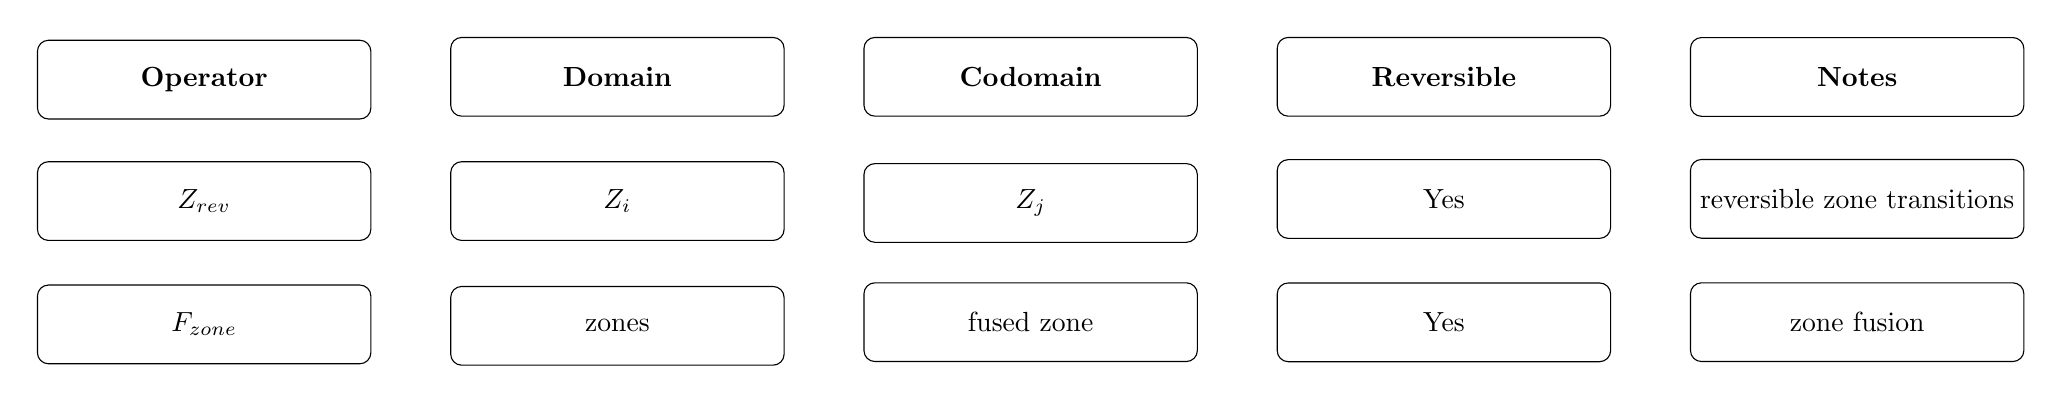
\begin{tikzpicture}
\matrix (m5) [matrix of nodes,
    nodes={draw, rectangle, rounded corners, align=center, text width=4cm, minimum height=1cm},
    column sep=1cm, row sep=0.5cm
]{
\textbf{Operator} & \textbf{Domain} & \textbf{Codomain} & \textbf{Reversible} & \textbf{Notes} \\
$Z_{rev}$ & $Z_i$ & $Z_j$ & Yes & reversible zone transitions \\
$F_{zone}$ & zones & fused zone & Yes & zone fusion \\
};
\end{tikzpicture}

\vspace{1cm}

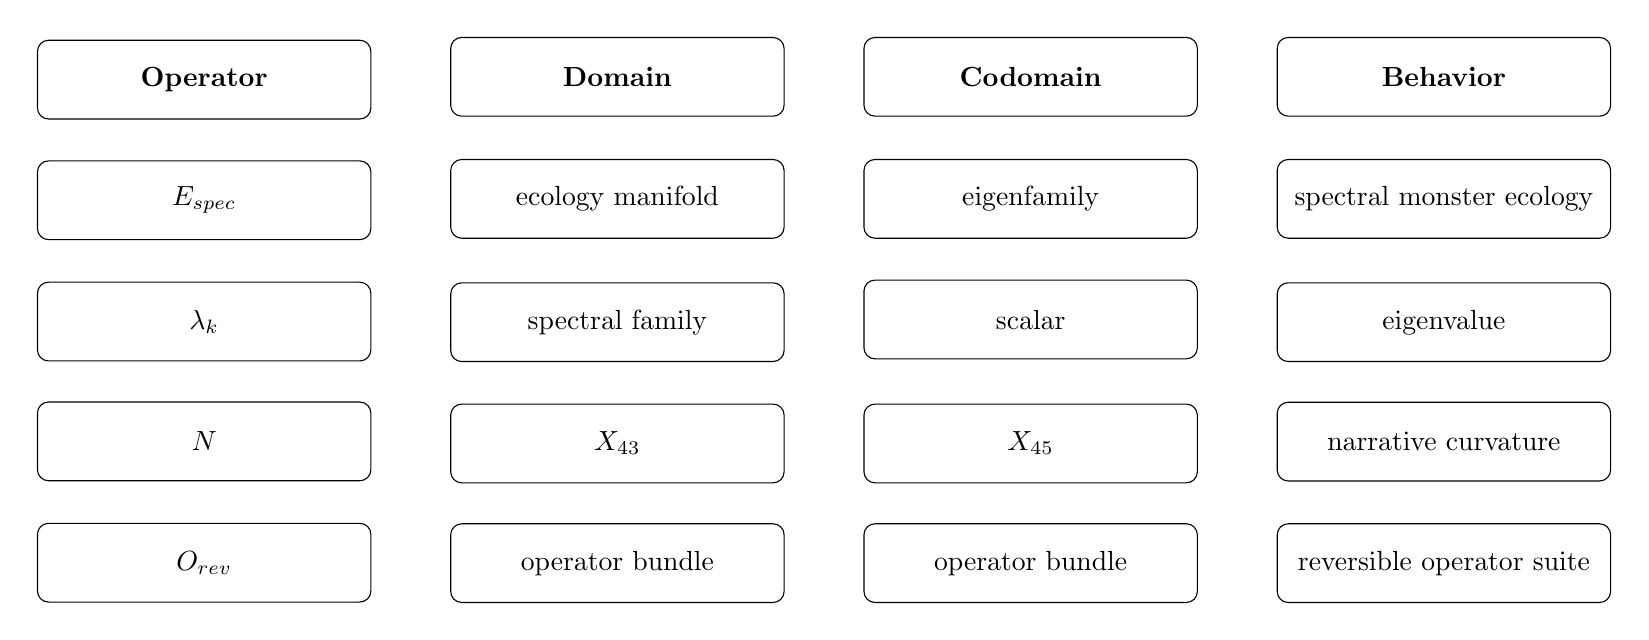
\begin{tikzpicture}
\matrix (m6) [matrix of nodes,
    nodes={draw, rectangle, rounded corners, align=center, text width=4cm, minimum height=1cm},
    column sep=1cm, row sep=0.5cm
]{
\textbf{Operator} & \textbf{Domain} & \textbf{Codomain} & \textbf{Behavior} \\
$E_{spec}$ & ecology manifold & eigenfamily & spectral monster ecology \\
$\lambda_k$ & spectral family & scalar & eigenvalue \\
$N$ & $X_{43}$ & $X_{45}$ & narrative curvature \\
$O_{rev}$ & operator bundle & operator bundle & reversible operator suite \\
};
\end{tikzpicture}

\vspace{1.5cm}

% ============================================================
% C.6 Collapse Behavior Summary
% ============================================================
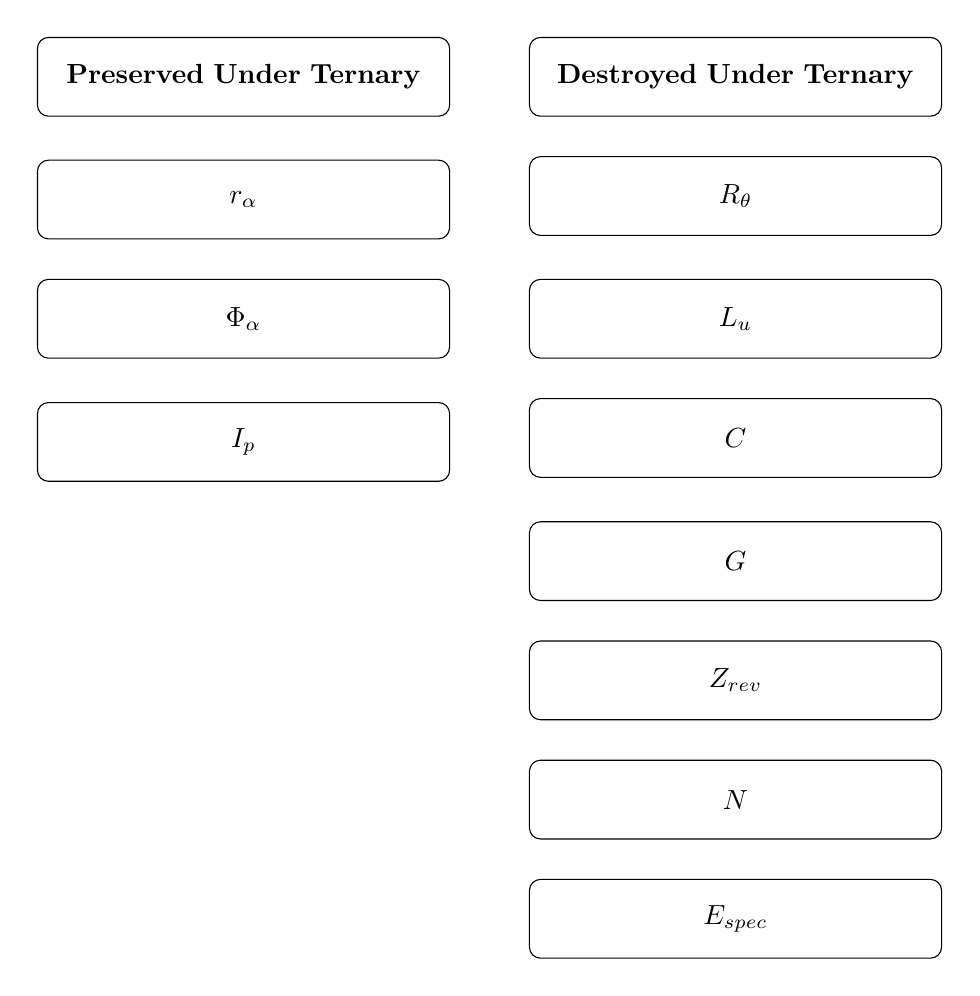
\begin{tikzpicture}
\matrix (m7) [matrix of nodes,
    nodes={draw, rectangle, rounded corners, align=center, text width=5cm, minimum height=1cm},
    column sep=1cm, row sep=0.5cm
]{
\textbf{Preserved Under Ternary} & \textbf{Destroyed Under Ternary} \\
$r_\alpha$ & $R_\theta$ \\
$\Phi_\alpha$ & $L_u$ \\
$I_p$ & $C$ \\
 & $G$ \\
 & $Z_{rev}$ \\
 & $N$ \\
 & $E_{spec}$ \\
};
\end{tikzpicture}

\vspace{1.5cm}

% ============================================================
% C.7 Altitude Requirements Summary
% ============================================================
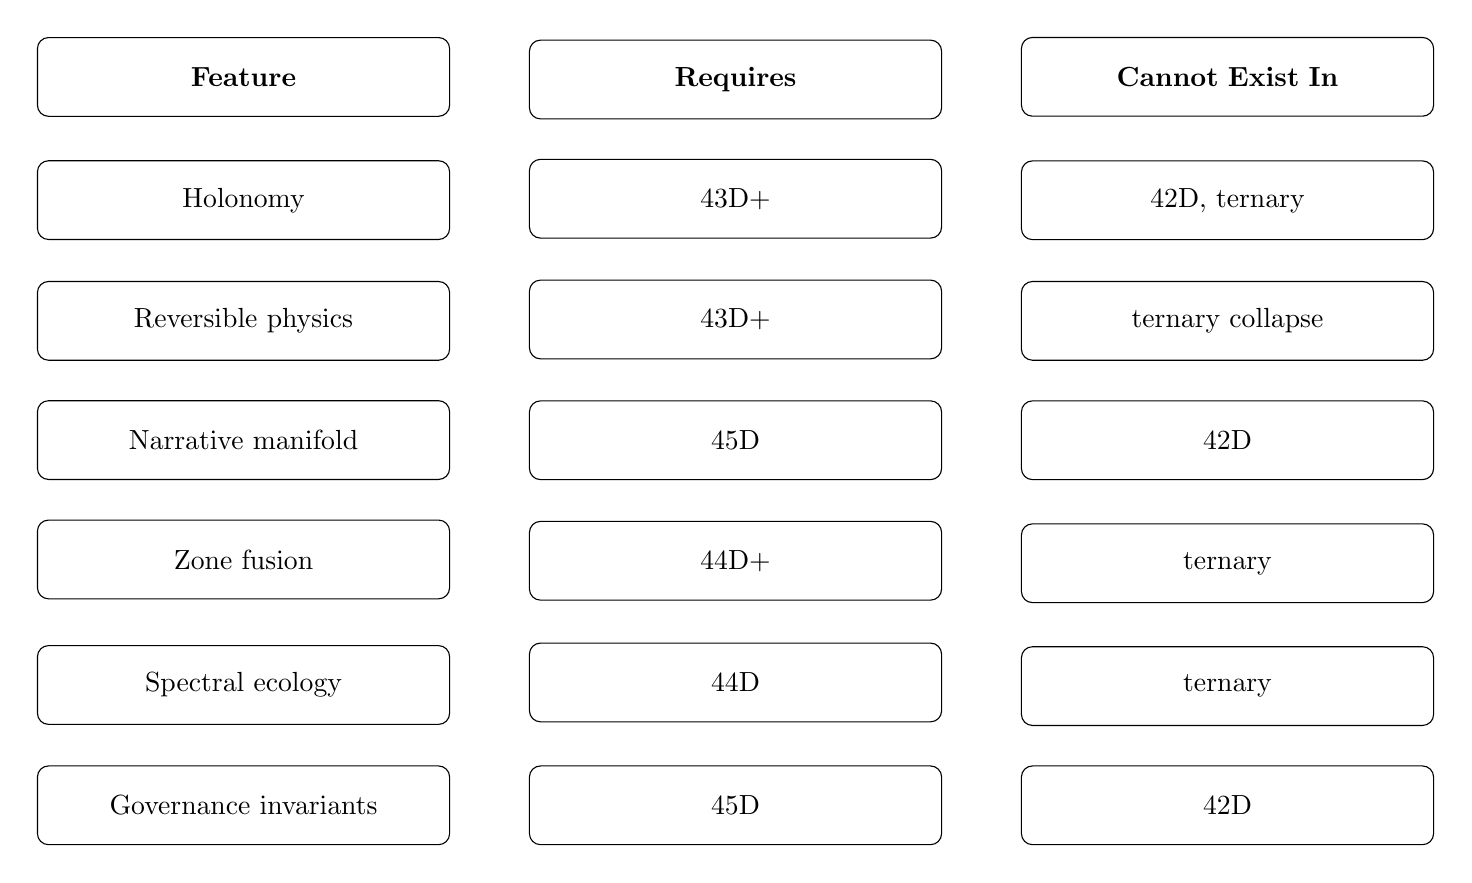
\begin{tikzpicture}
\matrix (m8) [matrix of nodes,
    nodes={draw, rectangle, rounded corners, align=center, text width=5cm, minimum height=1cm},
    column sep=1cm, row sep=0.5cm
]{
\textbf{Feature} & \textbf{Requires} & \textbf{Cannot Exist In} \\
Holonomy & 43D+ & 42D, ternary \\
Reversible physics & 43D+ & ternary collapse \\
Narrative manifold & 45D & 42D \\
Zone fusion & 44D+ & ternary \\
Spectral ecology & 44D & ternary \\
Governance invariants & 45D & 42D \\
};
\end{tikzpicture}

\vspace{1.5cm}

% ============================================================
% C.8 Conclusion (TikZ block)
% ============================================================
\begin{tikzpicture}
\node[draw, rectangle, rounded corners, align=center, text width=12cm, padding=10pt] {
Appendix C provides a complete operator-level reference for NDH and Fun-Sphere physics.\\[6pt]
42D operators are stable but non-expressive.\\
Ternary projection is diagnostic but destructive.\\
Fun-Sphere physics requires 43D–45D altitude operators.\\
Holonomy, reversibility, and narrative curvature cannot be represented in 42D.
};
\end{tikzpicture}

\end{document}
